\section{Discussion}

In the previous section, we have analysed the mechanisms of fish biomass response to interannual ENSO variability, focusing on the 97 El Nino event. We have seen that for large sizes, the biological processes have barely no impact on the fish biomass anomalies at interannual time-scales, which are solely driven by advection and diffusion processes.

However, several questions arise from the previous analysis. First, is the response to ENSO variability the dominant driver of biomass anomalies in the equatorial region? Second, in addition to the interannual response, is there a decadal response of marine ecosystems to ENSO variability?

In order to address these questions, fish biomass anomalies have been decomposed into Empirical Orthogonal functions, as described in section \ref{sec:eof}. EOFs have been computed in the 20N-20S, 150E-120W, in order to focus on the Equatorial Pacific region. Then, the EOF maps have been extended to the entire Pacific Ocean by computing the covariance maps between the PCs and the biomass anomalies. The resulting maps are shown in Fig\ref{fig:eofmaps} for the first two EOFs of small, intermediate and large sizes.

\begin{figure}
    \centering
    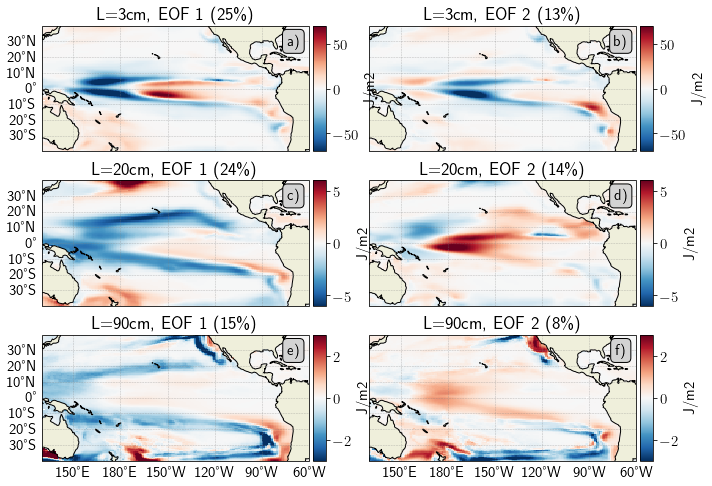
\includegraphics[width=\textwidth]{covariance_OOPE_pcs_latmax_20_lonmin_150_lonmax_-120_all_sizes.png}
    \caption{First two EOF maps of fish biomass anomalies for small (top), intermediate (middle) and large sizes.}
    \label{fig:eofmaps}
\end{figure}

The first EOF of small size fish biomass anomalies is very similar to the covariance maps shown in Fig\ref{fig:mean_ond97_ape}. This suggests that the interannual response to ENSO variability is the dominant mode of variability of small sizes, explaining 25\% of the total variance. This is further confirmed when comparing the first PC with the ONI index (Fig\ref{fig:eofpcs}a), which are strongly correlated (correlation coefficient of 0.80). The second principal component of small size classes ressembles the first EOF, but westward shifted and with opposite signs. Looking at PC2 suggests that this second EOF peaks during extreme El Nino events, such as 1982–83, 1997-98 and 2014-16. We interpret this pattern as a correction factor, whose effect would be to shift the pattern shown by EOF1 to the east for extreme El Ninos.

The first EOF of intermediate size-classes, which account for 24\% of the total variance, shows negative horseshoe-like anomalies. It somehow resembles the first EOF of small sizes, but with a poleward extension of the anomalies. Still, this pattern does not seem at first to be related with the ENSO variability. On the other hand, the second EOF, which explains 14\% of the total variance, closely resembles to the biomass anomalies associated with ENSO (Fig\ref{fig:mean_ond97_ape}). Investigating the principal components, we see that PC1 shows low-frequency variability, which varies in phase with the low-frequency PC index (correlation of 0.71 between PC1 and the filtered PCI index). PC2, on the other hand, shows interannual variability which varies and is strongly correlated with the ONI index (correlation of 0.75). Therefore, it seems that ENSO variability impacts intermediate fish biomass anomalies into two ways. First, the dominant impact occurs at decadal time-scales and might result from the integration, through predation, of the interannual response of small sizes, as discussed in \cite{lorenzoDoubleintegrationHypothesisExplain2013}. 

For large sizes, the first two EOFs explain a small amount of variance (15 and 8\%, respectively), and therefore this analysis might not as relevant as for small and intermediate sizes. Nevertheless, the first EOF seems to be the poleward extension of the first EOF of intermediate sizes. And the first principal component shows a decadal variability, but which seems to be lagged compared to the low-frequency TPI index. This seems to suggest that as size-increases, the period of the dominant mode of variability gets longer and the lag increases as well.

This is further confirmed in Fig.\ref{fig:pc_corrs}, which shows, for each size classes, the lead-lag correlations between the interannual PCI and decadal TPI indexes and PC1 of fish biomass anomalies, as well as the explained variance. Significance of the correlations have been inferred using a Student t-test. The number of degrees have been corrected following \cite{brethertonEffectiveNumberSpatial1999}.

Correlation between PC1 and the ONI index is strong for small size-classes ($<10 cm$) at 0-lags. As size increases, the strength of the correlation decreases and the lag increases. On the other hand, the correlation with the low pass filtered TPI index is low for small sizes, and increases with sizes but for lags greater than $\approx 10$ months.

\begin{figure}
    \centering
    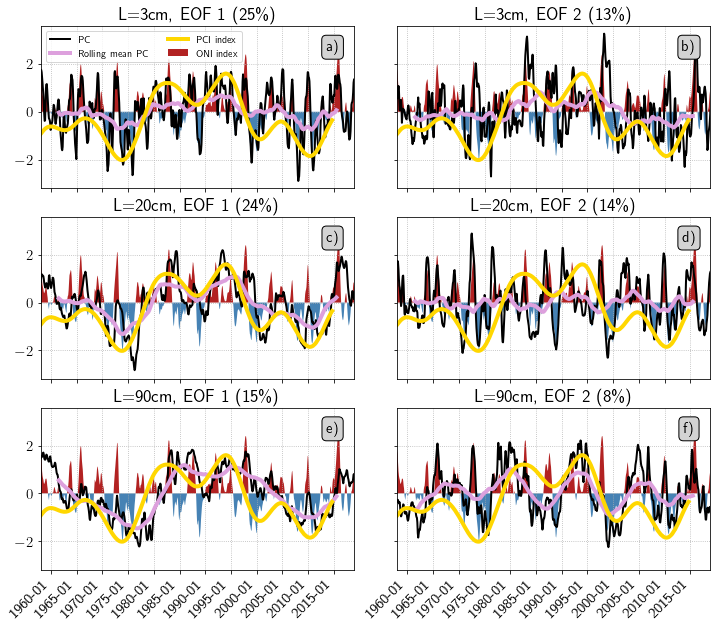
\includegraphics[width=\textwidth]{pcs_latmax_20_lonmin_150_lonmax_-120.png}
    \caption{First two EOF maps of fish biomass anomalies for small (top), intermediate (middle) and large sizes.}
    \label{fig:eofpcs}
\end{figure}


\begin{figure}
    \centering
    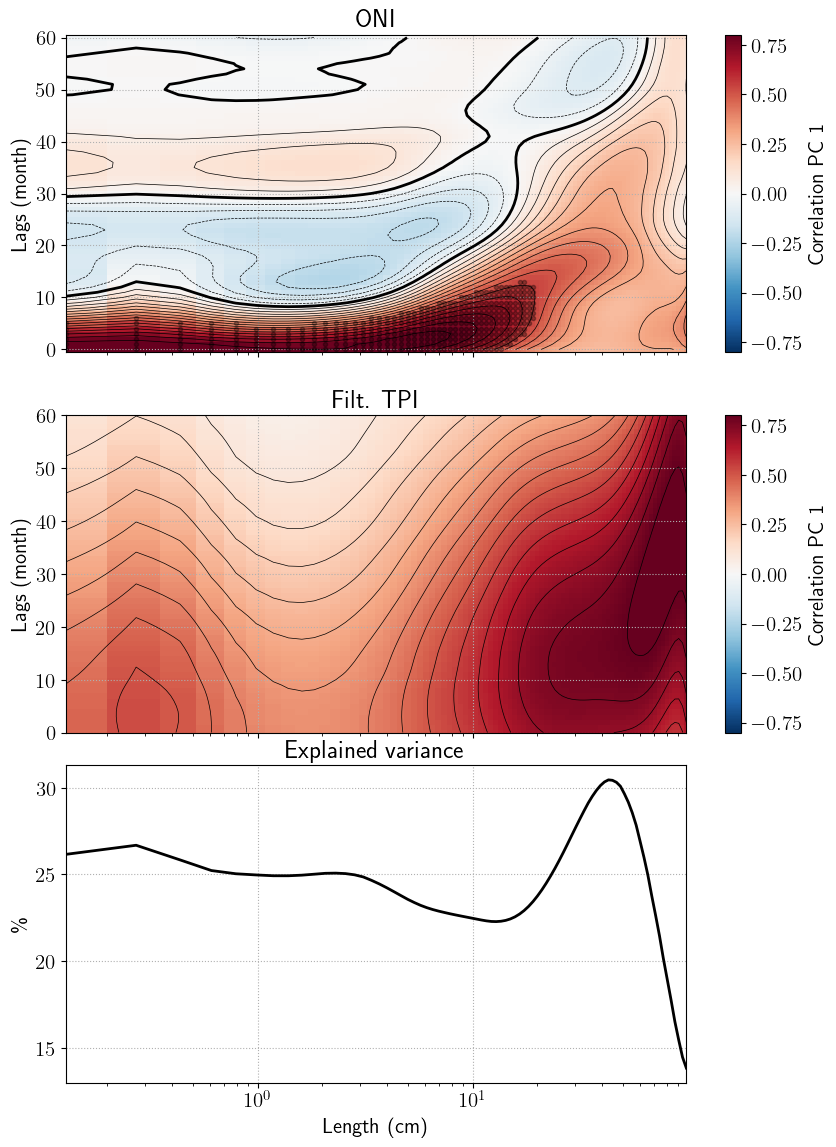
\includegraphics[scale=0.5]{figs/correlations_eof_oni_tpi_eof_1.png}
    \caption{Lead-lag correlations of PC1 with the ONI (top) and TPI (middle) indexes and explained variance as a function of length (log-scale).}
    \label{fig:pc_corrs}
\end{figure}

